\IfFileExists{stacks-project.cls}{%
\documentclass{stacks-project}
}{%
\documentclass{amsart}
}

% For dealing with references we use the comment environment
\usepackage{verbatim}
\newenvironment{reference}{\comment}{\endcomment}
%\newenvironment{reference}{}{}
\newenvironment{slogan}{\comment}{\endcomment}
\newenvironment{history}{\comment}{\endcomment}

% For commutative diagrams we use Xy-pic
\usepackage[all]{xy}

% We use 2cell for 2-commutative diagrams.
\xyoption{2cell}
\UseAllTwocells

% We use multicol for the list of chapters between chapters
\usepackage{multicol}

% This is generally recommended for better output
\usepackage{lmodern}
\usepackage[T1]{fontenc}

% For cross-file-references
\usepackage{xr-hyper}

% Package for hypertext links:
\usepackage{hyperref}

% For any local file, say "hello.tex" you want to link to please
% use \externaldocument[hello-]{hello}
\externaldocument[introduction-]{introduction}
\externaldocument[conventions-]{conventions}
\externaldocument[sets-]{sets}
\externaldocument[categories-]{categories}
\externaldocument[topology-]{topology}
\externaldocument[sheaves-]{sheaves}
\externaldocument[sites-]{sites}
\externaldocument[stacks-]{stacks}
\externaldocument[fields-]{fields}
\externaldocument[algebra-]{algebra}
\externaldocument[brauer-]{brauer}
\externaldocument[homology-]{homology}
\externaldocument[derived-]{derived}
\externaldocument[simplicial-]{simplicial}
\externaldocument[more-algebra-]{more-algebra}
\externaldocument[smoothing-]{smoothing}
\externaldocument[modules-]{modules}
\externaldocument[sites-modules-]{sites-modules}
\externaldocument[injectives-]{injectives}
\externaldocument[cohomology-]{cohomology}
\externaldocument[sites-cohomology-]{sites-cohomology}
\externaldocument[dga-]{dga}
\externaldocument[dpa-]{dpa}
\externaldocument[sdga-]{sdga}
\externaldocument[hypercovering-]{hypercovering}
\externaldocument[schemes-]{schemes}
\externaldocument[constructions-]{constructions}
\externaldocument[properties-]{properties}
\externaldocument[morphisms-]{morphisms}
\externaldocument[coherent-]{coherent}
\externaldocument[divisors-]{divisors}
\externaldocument[limits-]{limits}
\externaldocument[varieties-]{varieties}
\externaldocument[topologies-]{topologies}
\externaldocument[descent-]{descent}
\externaldocument[perfect-]{perfect}
\externaldocument[more-morphisms-]{more-morphisms}
\externaldocument[flat-]{flat}
\externaldocument[groupoids-]{groupoids}
\externaldocument[more-groupoids-]{more-groupoids}
\externaldocument[etale-]{etale}
\externaldocument[chow-]{chow}
\externaldocument[intersection-]{intersection}
\externaldocument[pic-]{pic}
\externaldocument[weil-]{weil}
\externaldocument[adequate-]{adequate}
\externaldocument[dualizing-]{dualizing}
\externaldocument[duality-]{duality}
\externaldocument[discriminant-]{discriminant}
\externaldocument[derham-]{derham}
\externaldocument[local-cohomology-]{local-cohomology}
\externaldocument[algebraization-]{algebraization}
\externaldocument[curves-]{curves}
\externaldocument[resolve-]{resolve}
\externaldocument[models-]{models}
\externaldocument[functors-]{functors}
\externaldocument[equiv-]{equiv}
\externaldocument[pione-]{pione}
\externaldocument[etale-cohomology-]{etale-cohomology}
\externaldocument[proetale-]{proetale}
\externaldocument[relative-cycles-]{relative-cycles}
\externaldocument[more-etale-]{more-etale}
\externaldocument[trace-]{trace}
\externaldocument[crystalline-]{crystalline}
\externaldocument[spaces-]{spaces}
\externaldocument[spaces-properties-]{spaces-properties}
\externaldocument[spaces-morphisms-]{spaces-morphisms}
\externaldocument[decent-spaces-]{decent-spaces}
\externaldocument[spaces-cohomology-]{spaces-cohomology}
\externaldocument[spaces-limits-]{spaces-limits}
\externaldocument[spaces-divisors-]{spaces-divisors}
\externaldocument[spaces-over-fields-]{spaces-over-fields}
\externaldocument[spaces-topologies-]{spaces-topologies}
\externaldocument[spaces-descent-]{spaces-descent}
\externaldocument[spaces-perfect-]{spaces-perfect}
\externaldocument[spaces-more-morphisms-]{spaces-more-morphisms}
\externaldocument[spaces-flat-]{spaces-flat}
\externaldocument[spaces-groupoids-]{spaces-groupoids}
\externaldocument[spaces-more-groupoids-]{spaces-more-groupoids}
\externaldocument[bootstrap-]{bootstrap}
\externaldocument[spaces-pushouts-]{spaces-pushouts}
\externaldocument[spaces-chow-]{spaces-chow}
\externaldocument[groupoids-quotients-]{groupoids-quotients}
\externaldocument[spaces-more-cohomology-]{spaces-more-cohomology}
\externaldocument[spaces-simplicial-]{spaces-simplicial}
\externaldocument[spaces-duality-]{spaces-duality}
\externaldocument[formal-spaces-]{formal-spaces}
\externaldocument[restricted-]{restricted}
\externaldocument[spaces-resolve-]{spaces-resolve}
\externaldocument[formal-defos-]{formal-defos}
\externaldocument[defos-]{defos}
\externaldocument[cotangent-]{cotangent}
\externaldocument[examples-defos-]{examples-defos}
\externaldocument[algebraic-]{algebraic}
\externaldocument[examples-stacks-]{examples-stacks}
\externaldocument[stacks-sheaves-]{stacks-sheaves}
\externaldocument[criteria-]{criteria}
\externaldocument[artin-]{artin}
\externaldocument[quot-]{quot}
\externaldocument[stacks-properties-]{stacks-properties}
\externaldocument[stacks-morphisms-]{stacks-morphisms}
\externaldocument[stacks-limits-]{stacks-limits}
\externaldocument[stacks-cohomology-]{stacks-cohomology}
\externaldocument[stacks-perfect-]{stacks-perfect}
\externaldocument[stacks-introduction-]{stacks-introduction}
\externaldocument[stacks-more-morphisms-]{stacks-more-morphisms}
\externaldocument[stacks-geometry-]{stacks-geometry}
\externaldocument[moduli-]{moduli}
\externaldocument[moduli-curves-]{moduli-curves}
\externaldocument[examples-]{examples}
\externaldocument[exercises-]{exercises}
\externaldocument[guide-]{guide}
\externaldocument[desirables-]{desirables}
\externaldocument[coding-]{coding}
\externaldocument[obsolete-]{obsolete}
\externaldocument[fdl-]{fdl}
\externaldocument[index-]{index}

% Theorem environments.
%
\theoremstyle{plain}
\newtheorem{theorem}[subsection]{Theorem}
\newtheorem{proposition}[subsection]{Proposition}
\newtheorem{lemma}[subsection]{Lemma}

\theoremstyle{definition}
\newtheorem{definition}[subsection]{Definition}
\newtheorem{example}[subsection]{Example}
\newtheorem{exercise}[subsection]{Exercise}
\newtheorem{situation}[subsection]{Situation}

\theoremstyle{remark}
\newtheorem{remark}[subsection]{Remark}
\newtheorem{remarks}[subsection]{Remarks}

\numberwithin{equation}{subsection}

% Macros
%
\def\lim{\mathop{\mathrm{lim}}\nolimits}
\def\colim{\mathop{\mathrm{colim}}\nolimits}
\def\Spec{\mathop{\mathrm{Spec}}}
\def\Hom{\mathop{\mathrm{Hom}}\nolimits}
\def\Ext{\mathop{\mathrm{Ext}}\nolimits}
\def\SheafHom{\mathop{\mathcal{H}\!\mathit{om}}\nolimits}
\def\SheafExt{\mathop{\mathcal{E}\!\mathit{xt}}\nolimits}
\def\Sch{\mathit{Sch}}
\def\Mor{\mathop{\mathrm{Mor}}\nolimits}
\def\Ob{\mathop{\mathrm{Ob}}\nolimits}
\def\Sh{\mathop{\mathit{Sh}}\nolimits}
\def\NL{\mathop{N\!L}\nolimits}
\def\CH{\mathop{\mathrm{CH}}\nolimits}
\def\proetale{{pro\text{-}\acute{e}tale}}
\def\etale{{\acute{e}tale}}
\def\QCoh{\mathit{QCoh}}
\def\Ker{\mathop{\mathrm{Ker}}}
\def\Im{\mathop{\mathrm{Im}}}
\def\Coker{\mathop{\mathrm{Coker}}}
\def\Coim{\mathop{\mathrm{Coim}}}

% Boxtimes
%
\DeclareMathSymbol{\boxtimes}{\mathbin}{AMSa}{"02}

%
% Macros for moduli stacks/spaces
%
\def\QCohstack{\mathcal{QC}\!\mathit{oh}}
\def\Cohstack{\mathcal{C}\!\mathit{oh}}
\def\Spacesstack{\mathcal{S}\!\mathit{paces}}
\def\Quotfunctor{\mathrm{Quot}}
\def\Hilbfunctor{\mathrm{Hilb}}
\def\Curvesstack{\mathcal{C}\!\mathit{urves}}
\def\Polarizedstack{\mathcal{P}\!\mathit{olarized}}
\def\Complexesstack{\mathcal{C}\!\mathit{omplexes}}
% \Pic is the operator that assigns to X its picard group, usage \Pic(X)
% \Picardstack_{X/B} denotes the Picard stack of X over B
% \Picardfunctor_{X/B} denotes the Picard functor of X over B
\def\Pic{\mathop{\mathrm{Pic}}\nolimits}
\def\Picardstack{\mathcal{P}\!\mathit{ic}}
\def\Picardfunctor{\mathrm{Pic}}
\def\Deformationcategory{\mathcal{D}\!\mathit{ef}}

%Dani's additions
\usepackage{graphicx} %figures


\begin{document}

\title{Differential Geometry}
\maketitle

\phantomsection
\label{section-phantom}

\tableofcontents

\section{Geodesics}
\label{section-geodesics}

\begin{proposition}[Totally Normal Neighbourhoods]
\label{proposition-totally-normal-neighbourhoods}
For all $p \in M$ there is a neighbourhood $W \ni p$ and a number $\delta>0$ 
 such that for every $q \in W$, $B_\delta(q)$ is normal and
 $W \subset B_\delta(q)$. 
\end{proposition}

\section{Jacobi Fields}
\label{section-jacobi-fields}

\begin{proposition}[Everyday Jacobi field]
\label{proposition-everyday-jacobi-field}
\cite{doc} Chapter V, Proposition 2.4. Let $\gamma:[0,a]\to M$ be a normalized
geodesic and let $J$ be a Jacobi field through $\gamma$ with $J(0)=0$.
Let $p:=\gamma(0)$ $w:=J'(0)$ and  $v:=\gamma'(0)$. 
Consider the variation
$$
f(s,t):=\operatorname{exp}_{p}(t(v+sw))
$$
Then the associated Jacobi field is $J$. So in particular the field
$$
J(t)=d_{tv}\operatorname{exp}_p(tw)
$$
is a Jacobi field.

{\bf Remark:} the variation can also be taken with respect to
any a curve $\sigma$ on $T_vT_{p}M$ passing through $v$ 
at $s=0$ with velocity $w$.

\end{proposition}

\begin{example}[Jacobi Fields in constant curvature]
\label{example-jacobi-fields-in-constant-curvature}
If $M$ has constant curvature $k$, a Jacobi field is of the form
\end{example}

\begin{proposition}[Critical points of exponential]
\label{proposition-critical-points-exp}
\cite{doc} Chapter V, Proposition 3.5. A vector $v \in T_pM$ is a critical
point of $\operatorname{exp}_p$ if and only if the corresponding 
$\gamma_v(1)$ is a conjugate point of $p$ along $\gamma_v$.
Moreover, in such points, the dimension of the kernel of 
$\operatorname{exp}_p$ at this vector is the multiplicity
of the conjugate point $\gamma_v(1)$ 
(i.e. the dimension of the space of Jacobi fields vanishing 
at the endpoints).
\end{proposition}

\begin{proof}
($\implies$) Suppose that $v$ is a critical point of $\operatorname{exp}_p$ and 
let $w \in \ker d_v \operatorname{exp}_p$ then a Jacobi field along $\gamma$ 
vanishing at the endpoints is given by
$$
J(t):=d_{tv}\operatorname{exp}_ptw
$$
($\impliedby$) If you have a critical point along $\gamma$, then the 
differential of $\operatorname{exp}_p$ has kernel.

(Mulitplicity.) The proof every element of the kernel gives a Jacobi
 field vanishing at the points. Linearly dependent elements will give 
 linearly dependent Jacobi fields.
\end{proof}
\section{Submanifolds}
\label{section-submanifolds}

\begin{remark}
\label{remark-ricci-equation}
Ricci equation may help prove that the normal bundle of a high codimension
submanifold is trivial.
\end{remark}

\section{Hopf-Rinow Theorem}
\label{section-Hopf-Rinow-theorem}

\begin{theorem}[Hopf-Rinow]
\label{theorem-Hopf-Rinow}
The following are equivalent for any $p \in M$:
\begin{enumerate}
\item The domain of the exponential map $\text{exp}_p$ is $T_pM$.
\item Closed and bounded subsets are compact.
\item $(M,d)$ is a complete metric space.
\item $M$ is geodeiscally complete (i.e. every geodesic is maximally defined in
all of $\mathbb{R}$).
\item Existence of exhaustions.
\end{enumerate}
Moreover, each of the former conditions imply that there exists a minimizing 
geodesic joining any two points.
\end{theorem}
\section{First Variation Formula}
\label{section-first-variation}

\begin{theorem}[First Variation Formula]
\label{theorem-first-variation-formula}
If  $f:(-\varepsilon,\varepsilon)\times(-\delta,\delta) \to M$ is a variation of
the geodesic $\gamma(-\delta,\delta)\to M$, then
$$
\frac{1}{2}E'(0)=-\int_a^b\left<V,\gamma''\right>+\left<V,\gamma'\right>|_{a}^b
+\sum_{i=1}^{k-1}\left<V,\gamma'^{-}(t_{i})-\gamma'^{+}(t_i)\right>
$$
\end{theorem}

\section{Second Variation Formula}
\label{section-second-variation}


\section{Bonnet-Myers Theorem}
\label{subsection-Bonnet-Myers-theorem}

\begin{theorem}[Bonnet-Myers]
\label{theorem-bonnet-myers}
If $M$ is a complete manifold with $\operatorname{Ric} \geq \frac{1}{r^2}$, then
$\operatorname{diam}M\leq \pi r$. In particular, $M$ is compact.
\end{theorem}

\section{Rauch's comparison theorem}
\label{section-Rauch}

\section{Weinstein's theorem}
\label{section-Weinstein-theorem}

\begin{theorem}[Weinstein]
\label{theorem-Weinstein}
Let $M^n$ be oriented, compact, $K>0$ and $f \in \text{Iso}(M)$. Suppose that 
if $n$ is even, $f$ preserves orientation, and if $n$ is odd, $f$ reverts
orientation. Then $f$ has a fixed point.
\end{theorem}

\section{Synge's theorem}
\label{section-Synge-theorem}

\begin{theorem}[Synge]
\label{theorem-Synge}
Let $M^n$ be compact and $K>0$. Then
\begin{enumerate}
\item If $n$ is even,
$$
\pi_1(M)=\begin{cases}
	1\qquad & \text{if $M$ is orientable}\\
	\mathbb{Z}_2\qquad & \text{if $M$ is not orientable}
\end{cases}
$$
\item If $n$ is odd, then $M^n$ is orientable.
\end{enumerate}
\end{theorem}

\begin{proof}
First suppose $n$ is even and $M$ is orientable. Since $M$ is compact we must
have that $K\geq \delta>0$. Now consider the universal cover $\tilde{M}$. Then
it also satisfies the curvature bound (with the pullback metric)
, making it compact as well by Bonnet-Myers \ref{theorem-bonnet-myers}. 
Now pick a deck transformation, which must be
orientation-preserving if we choose the orientation on $\tilde{M}$ (simply
connected is always orientable) making the projection orientation-preserving.
Then $f$ must have a fixed point by Weinstein's theorem \ref{theorem-Weinstein},
which applies since we have shown that $\tilde{M}$ is compact. 
However, deck transformations cannot have fixes points unless they are the
 identity: this is a consequence of the ``Unique lifting property", which a 
slightly more general statement than the uniqueness of curve lifts that we 
used for Klinenberg's lemma exercise \ref{exercise-l7-1}. 
More exactly (cf. \ref{proposition-unique-lifting-property}): 
given a covering space and to maps from any space into the base, these coincide
 if they agree at one point only.
\end{proof}

\section{Index lemma}
\label{subsection-index-lemma}

\section{Teorema de Rauch}
\label{subsection-Rauch}

\begin{theorem}[Rauch]
\label{theorem-Rauch}
\end{theorem}

\begin{proposition}
\label{proposition-contraction}
Sejam $p \in M$, $\tilde{p} \in \tilde{M}$ e $i:T_pM \to T_{\tilde{p}}\tilde{M}$
uma isometria. Então $f:=\operatorname{exp}^{-1}_p \circ i \circ
\operatorname{exp}_{\tilde{p}}$ é uma contração métrica, i.e. $|f_*w|\leq |w|$
para todo $w \in T_pM$.

Mas ainda, se $\operatorname{exp}_p^{-1}$ está definida numa bola totalmente
convexa, $f$ é uma contração métrica.
\end{proposition}

\begin{proof}
Write an abitrary $w\in T_p M$ as a Jacobi variational field of the variation 
$f(s,t)=\operatorname{exp}_p(t(v+sw)$. The resulting field on $\tilde{M}$ is a
Jacobi field with respect to $iw$ using that $i$ is an isometry. The conditions
of Rauch theorem are satisfied and the desired inequality is obtained.

For the metric result we just integrate along a curve realising the distance and
compute.
\end{proof}

\section{Morse index theorem}
\label{section-morse-index}

\begin{definition}[Index of index form]
\label{definition-index-index-form}
$$
i(I_a):=\operatorname{sup}\{\dim L \subset \mathfrak{X}_\gamma:I_a |_{L \times L}<0\}
$$
\end{definition}


\begin{theorem}[Morse Index]
\label{theorem-morse-index}
O índice $i(I_t)$ é finito e igual ao número de pontos conjugados em $[0,t)$ ao
longo de $\gamma$.
\end{theorem}

\begin{proof}
\begin{enumerate}
\item Define
\begin{align*}
\mathcal{V}_a&=\{V \in \mathfrak{X}_\gamma:\text{d.p.p., }V(0)=0, V(a)=0\}\\
\mathcal{V}_t^+&:=\{V \in \mathcal{V}_t:V(t_i)=0\}\\
\mathcal{V}_t^-& :=\{V \in \mathcal{V}_t:V|_{[t_j,t_{j+1}]}\in
\mathfrak{X}_{\gamma|_{[t_j,t_{j+1}]}}^J\}
\end{align*}
\item Note que
$$
\mathcal{V}_t=\mathcal{V}_t^+ \oplus  \mathcal{V}_t^-
$$
\item Note que 
$$
\mathcal{V}_t^-=\bigoplus_{j=1}^{i-1}T_{\gamma(t_j)}M
$$
porque para qualquer escolha de vetores
 $v_1 \in T_{\gamma(t_1)}M,\ldots,v_{i-1}\in T_{\gamma(t_{i-1})}M$ existe
 um único campo $J \in \mathcal{V}^-$ tal que $J(t_j)=v_j$, por ser a solução
 da EDO com condições de contorno.
\item (\cite{doc} Capítulo X, Proposição 2.3. A nulidade da forma do índice é
$$
\Ker I_t:=\{V \in \mathcal{V}_t:I_t(V,W)=0\forall W\in\mathcal{V}_t\}=
V_t \cap \mathfrak{X}_\gamma^J 
$$
The point here is to show that if $V \in \Ker$ then it is (1) a Jacobi
 field in each interval where $V$ is smooth, and (2) smooth in the whole
 interval.

We use the fact that $V$ is in the kernel to show that (1) the norm of 
$V-R_{\gamma'}V$ is zero, and (2) the left and right derivatives of $V$
coincide. The first part involves multiplying by a positive function $f$ that
vanishes at the singular points; this will make the ``singular part" of the
index form, i.e. the sum, vanish, so that we get only with the integral part,
which is the norm of the Jacobi equation, which will vanish since we are in the
kernel. The second part I'm not sure---why do we need to show that $V$ is
differentiable, or $C^2$ (since it's the solution of an ODE).
\end{enumerate}
\end{proof}

\section{Cut locus}
\label{section-cut-locus}

\begin{definition}[Cut point]
\label{definition-cut-point}
O {\it cut point} de  $p$ ao longo de $\gamma$ é $\gamma(\rho(\gamma))$ 
onde
$$
\rho(\gamma)=\text{sup}\{t:\gamma|_{[0,t]}\text{ é minimizante}\}
$$

\end{definition}

\begin{proposition}[Cut point characterization]
\label{proposition-cut-point-characterization}
\cite{doc} Chapter XIII, Proposition 2.2. Let $\gamma$ be a minimizing geodesic joining $p$ and $q$. Then $q$ is the cut
point of $p$ if and only if either of the following conditions hold:
\begin{enumerate}
\item $q$ is the first conjugate point of $p$ along $\gamma$.
\item There is another, distinct, minimizing geodesic $\sigma$ joining $p$ and
 $q$.
\end{enumerate}
\end{proposition}

\begin{proof}[Sketch of proof]
($\implies$) Since $q:=\gamma(r)$ is the cut point of $p$, we know that for every point
$\gamma(r+\varepsilon)$ along $\gamma$ after $q$ there must be some other geodesic
$\gamma_\varepsilon$ which realizes the distance between $p$ and
$\gamma(r+\varepsilon)$

Taking the limit as $\varepsilon \to 0$ we obtain another geodesic
(because we are taking limit inside $S^n \subset T_pM$, so we get convergence;
and because ``things will behave well under the limit")
which puts us in the second condition of the theorem,
unless the limit geodesic is the same as  $\gamma$ setwise.

Now there's a critical observation:
the two geodesics $\gamma$ and $\gamma_\varepsilon$ meet at the point 
 $\gamma(r+\varepsilon)$, so you can write
 $\gamma_\varepsilon(r+\delta(\varepsilon))=\gamma(r+\varepsilon)$
 for some function $\delta(\varepsilon)$ (that could be negative, doesn't
 matter).
 But since $\gamma_\varepsilon$ is the minimizing
 geodesic from $\gamma(0)$ to this point, then
 $|\delta(\varepsilon)|<\varepsilon$.

Right, the point is that defining
$$
u_\varepsilon:=(r+\varepsilon)v,\qquad
u'_\varepsilon:=r+\delta(\varepsilon))v_\varepsilon
$$
we see that $\operatorname{exp}_p$ is not injective, since these two vectors
hit that point.

This being true for every $\varepsilon>0$, there is no neighbourhood of $vr$ 
where $\operatorname{exp}_p$ is injective---much less a diffeomorphism.
So it cannot be a local diffeomorphism, and we know that critical points of
$\operatorname{exp}_p$ are conjugate points of $p$. (Remember: if
$\operatorname{exp}_p$ has a critical point, its differential has kernel,
and the map $d_{tv}\operatorname{exp}_pw$, for $w$ in the kernel, gives 
a Jacobi field. See Proposition \ref{proposition-critical-points-exp})
\end{proof}

\begin{exercise}[Diâmetros]
\label{exercise-diametros}
Calcule o diâmetro de $S^2$, $\mathbb{T}^2$, $\mathbb{R}P^{2}$.
\end{exercise}

\begin{proof}[Solution]
O diâmetro de $S^2$ pode ser calculado via o teorema de Bonnet Myers
\ref{theorem-bonnet-myers}: nenhuma geodésica é minimizante depois de atingir
comprimento $\pi r$, e temos uma geodésica que atinge esse comprimento: qualquer
uma!

O diâmetro de $\mathbb{T}^2$ é $1$. Isso é por simples geometria
euclidiana: é o diâmetro do cubo! Por definição, a métrica de  $\mathbb{T}^2$ é
a induzida pela projeção quociente.

O diâmetro de $\mathbb{R}P^{2}$ é $\pi/2$. Qualquer geodésica que liga dois
pontos a distância $\pi/2$ é minimizante, pois estamos na métrica esférica e
podemos pegar cartas esféricas onde dois pontos a essa distância estão contidos. 
Por outro lado, se tivéssemos dois pontos a distância maior, a geodésica 
esférica que percorre o ponto antípoda ao inicial, chega no ponto final mais 
rapidamente que inicial; portanto geodésicas de comprimento maior que $\pi/2$ 
não são minimizantes.
\end{proof}

\begin{lemma}[Cut point is reflexive]
\label{lemma-cut-point-reflexive}
If $q$ is the cut point of $p$ through $\gamma$, then $p$ is the cut point of
$p$ through $\gamma$.
\end{lemma}

\begin{lemma}[Not in the cut locus implies minimizing]
\label{lemma-not-cut-locus-minimizing}

\end{lemma}

\begin{proposition}[Distance to cut point is continuous]\leavevmode
The function
\begin{align*}
	\rho: T^1_p &\longrightarrow [0,+\infty] \\
	v &\longmapsto \text{cut point along }\gamma_v 
\end{align*}
is continuous.
\end{proposition}

\begin{lemma}[Cut locus is a closed set]
\label{lemma-cut-locus-closed}
Because it's the image of the unit sphere in $T_pM$, which is closed.
\end{lemma}

\begin{lemma}[Cut locus is open, dense, homeomorphic to a ball, total measure]
\label{lemma-cut-locus-topology}

\end{lemma}

\begin{lemma}[Outside the cut locus implies exists unique minimizing geodesic]
\label{lemma-outside-cut-locus-exists-minimizing-geodesic}
\cite{doc} Chapter XIII, Corollary 2.8. If $q \in M\setminus C_m(p)$, there exists a
 unique minimizing geodesic joining
$p$ and $q$.
\end{lemma}

\begin{proof}
By Hopf-Rinow \ref{theorem-Hopf-Rinow}, we know that
there exists a minimizing geodesic joining any two points. If there was more
than one such geodesic, by 
Proposition \ref{proposition-cut-point-characterization} 
we get that $q$ is the cut point of  $q$ along either of these geodesics, 
a contradiction.
\end{proof}

The former Lemma \ref{lemma-outside-cut-locus-exists-minimizing-geodesic} 
shows that the exponential map $\text{exp}_p$
 is injective outside the cut locus of $p$. 
This motivates the following definition.

\begin{definition}[Injectivity radius]
\label{definition-injectivity-radius}
The {\it injectivity radius} of a manifold $M$ is
$$
i(M)=\operatorname{inf}\{d(p,C_m(p)):p \in M\}
$$
\end{definition}

\section{Bishop-Gromov Theorem}
\label{section-bishop-gromov}

\begin{theorem}[Bishop-Gromov]
\label{theorem-bishop-gromov}

\end{theorem}

\begin{proof}
Tome a função exponencial como uma carta parametrizando a esfera geodésica de
raio $r$ com centro em $p$. Então
$$
\operatorname{Vol}_{S_r}=\int
\operatorname{Vol}_{S_r}=
\int_{S_r(0)}\operatorname{exp}_p^*\operatorname{Vol}_{S_r}
$$
Portanto, estamos interessados em calcular 
$$
|\det d_{rv} \operatorname{exp}_p|
$$
Avaliando em uma base de vetores tangentes a $S_r(0)$, notamos que cada um deles
nos dá um campo de Jacobi $J$ ao longo de $\gamma$.

Como $\gamma'(r)\perp J$, derivando obtemos $A J=J'$ onde $A$ é o operador de
forma de $S_r$ respeito ao normal interior $\gamma'(r)$ (cf. conta feita antes).

Mmm… no sé: creo que lo que quiero calcular realmente es
$$
\det J
$$
entonces no sé dondé entran ni $A$ ni $J'$… O sea si derivas con respecto a $r$
pues va… pero si no…

\end{proof}

\section{Toponogov's theorem}
\label{section-Toponogov}

First recall

\begin{theorem}[Toponogov, local version]
\label{theorem-Toponogov,local}
Let $o,p_1,p_2 \in B$ where $B$ is a totally convex ball of $M$. Let $\gamma_1$
and $\gamma_2$ be the normalized geodesics joining $o$ to $p_1$ and to $p_2$.

Suppose $\tilde{o}, \tilde{p}_1,\tilde{p}_2 \in \tilde{B}$ is a triple on 
another manifold $\tilde{M}$ such that the distances from $\tilde{o}$ to
$\tilde{p}_1$ and from $\tilde{o}$ to $\tilde{p}_2$ coincide with those in $M$.

Then for any $t \in [0,\ell(\gamma_1)]$ and $s \in [0,\ell(\sigma)]$,
$$
\tilde{d}(\tilde{\gamma}_1(t),\tilde{\gamma}_s)\leq d(\gamma_1(t),\gamma_2(s))
$$
\end{theorem}

\begin{exercise}[Lista 7]
\label{exercise-Toponogov-from-Rauch}
Prove the local version of Toponogov's theorem as a corollary of Rauch's
Comparison Theorem \ref{theorem-Rauch}.
\end{exercise}

\begin{proof}
This is an application of Proposition \label{proposition:contraction} for $i$ as
given by the condition of mapping $\gamma'_1(0)$ to $\gamma_2'(0)$ and the angle
between them to the corresponding vectors and angle on $\tilde{M}$.
\end{proof}

\begin{theorem}[Toponogov, hinge version] \label{theorem-Toponogov-hinge}
Let $M$ be a complete manifold and $K \geq k$. Let $o,p_1,p_2 \in M$, with
$p_1\neq  p_2$. Let $\gamma_1$ and $\gamma_2$ be normalized geodesics joining 
$o$ to $p_1$ and to $p_2$. Suppose $\gamma_1$ is minimizing.
Let $\gamma_0$ be a nonconstant geodesic joining $p_1$ to $p_2$ and suppose
$$
\ell(\gamma_0) \leq \ell(\gamma_1) +\ell(\gamma_2)
$$
If $k>0$ suppose additionally that $\ell(\gamma_0) \leq \pi/\sqrt{k}$.

Then there exists a geodesic triangle $\{\tilde{\gamma}_i:i=1,2,0\}$ in
$\mathbb{Q}_k^2$ such that $\ell(\tilde{\gamma}_i) = \ell(\gamma_i)$ and
$$
d(\tilde{p}_1,\tilde{p}_2) \leq  d(o,p_1)+d(o,p_2)
$$

Put another way (next lecture…) Let $\tilde{\gamma}_1$ and $\tilde{\gamma}_2$ 
be a corresponding angle in $\mathbb{Q}_k^2$. Then
$$
\tilde{d}(\tilde{\gamma}_1(t),\tilde{\gamma}(s)\leq d(\gamma_1(t),\gamma_2(s))
$$

\end{theorem}

\begin{remark}
For me a more geometric statement is



Suppose $\tilde{o}, \tilde{p}_1,\tilde{p}_2 \in \tilde{B}$ is a triple on 
another manifold $\tilde{M}$ such that 
$$
d(\tilde{p}_1,\tilde{p}_2) \leq  d(o,p_1)+d(o,p_2)
$$
If the sectional curvature $K$ of $M$ is $K>0$, then suppose additionally that
$\ell(\gamma_1$

Then for any $t \in [0,\ell(\gamma_1)]$ and $s \in [0,\ell(\sigma)]$,
$$
\tilde{d}(\tilde{\gamma}_1(t),\tilde{\gamma}(s)\leq d(\gamma_1(t),\gamma_2(s))
$$
So it's the same right? You look form $p_1$ instead…
\end{remark}

\section{Gromov's theorem}
\label{section-Gromov-theorem}

\begin{theorem}[Gromov]
\label{theorem-Gromov}
$M^n$ complete, $K \geq 0$, then $\pi$ admits a set of $3^n$ generators. In
particular, it is finitely generated.
\end{theorem}

\begin{proof}
Consider the universal cover $\tilde{M}$ of $M$ with the pullback metric. Fix a
point $x \in \tilde{M}$ and consider the set
$$
\{f \in \Gamma:d(x,f(x))<r\},\qquad r>0
$$
By \ref{proposition-deck-transformations-act-properly-discontinuous}
every point must have a disjoint neighbourhood … 
\end{proof}

\section{Cartan's Theorem}
\label{section-Cartan-theorem}

\begin{definition}
\label{definition-free-homotopy-set}
The {\it free homotopy set} is the set of homotopy classes of loops based on any
point of $M$.
\end{definition}

\begin{definition}
\label{definition-geodesic-loop}
A {\it geodesic loop} is a geodesic whose starting and ending points are the
same. It may not be differentiable at such point.
\end{definition}

\begin{definition}
\label{definition-closed-geodesic}
A {\it closed geodesic} a smooth geodesic loop.
\end{definition}

\begin{theorem}[Cartan]
\label{theorem-Cartan}
Let $M^n$ be compact, and $\omega \in \hat{\pi}_1M$ nontrivial. Then there is a
closed geodesic $\gamma$ such that $[\gamma]=\omega$.
\end{theorem}

\begin{proof}
Consider a sequence of loops whose lengths converge to the number
$$
\ell:=\text{inf}\{\ell(c):c \in \omega\}>0
$$
Consider a sequence $c_n$ of curves in $\omega$ such that their lengths converge
to $\ell$. Then apply Arzelà-Ascoli Theorem \ref{theorem-Arzela-Ascoli}
 to ensure they converge to some curve $c$ and show this is a geodesic 
in $\omega$.

First suppose that each of the $c_n$ is a piecewise geodesic parametrized by
arclength (why can we do this?). We may then pick the supremum $L$ of all the
lengths since we are assuming that their lengths decrease. Then
$$
d(c_n(t),c_n(s)) \leq \ell \left(c_n|_{[t,s]}\right) \leq  N |t-s|
$$
This says that $\{c_n\}$ is equicontinuous (the same $N$ works for all $n$) as a
family of maps from 
\end{proof}

\section{Exercises}
\label{section-exercises}

\begin{exercise}[Geodésica sem pontos conjugados é localmente minimizante]
\label{exercise-geodesica-sem-pontos-conjugados-e-localmente-minimizante}
$\gamma$ geodésica sem pontos conjugados em $[0,a]$. Então $\gamma$ é localmente
minimizante.
\end{exercise}

\begin{proof}
Temos dois casos:
\begin{enumerate}
\item Se $E''(0)<0$ usamos o teorema do índice. Isto é, não é possível que
 $E''(0)<0$ porque isso implica que o índice da forma do índice é diferente
 de zero, ou seja, existem pontos conjugados.
\item Se $E''(0)=0$,
\begin{enumerate}
\item[(0)] Como $\gamma$ não tem pontos conjugados, então $I$ não tem
nulidade em todo  $\mathcal{V}$.
\item $I_{\mathcal{V}^-}$ não tem índice nem nulidade. Segue do ponto anterior + 
algum passo na prova.
\item $I_{\mathcal{V}^-}$ não tem índice.
\item 2+3 dão que $I_{\mathcal{V}^-}>0$.
\item Logo $I>0$.
\end{enumerate}
\end{enumerate}
\end{proof}

\begin{exercise}[Warped product]
\label{exercise-wraped-product}
Para $(M,g_M)$ e $(N,g_N)$ e $f:M \to \mathbb{R}_+$, definimos o {\it warped
product} como sendo o produto cartesiano $M\times N$ com a métrica 
 $g_M+f^2g_N$.

Mostre que se os fatores são completos, o warped product é completo.
\end{exercise}

\subsection{Highlight exercises}
\label{subsection-highlight-exercises}
\begin{exercise}
\label{exercise-minimal-intersection}
$(M^n,g)$ completa $\operatorname{Ric}_M>0$. $A$, $B$ hipersuperfícies mínimas
completas. Então  $A \cap B \neq \emptyset$.
\end{exercise}

\begin{proof}
Suponha que existe uma $\gamma$ mínima com comprimento positivo ligando as 
duas variedades. Tem dois caminhos:
\begin{enumerate}
\item Deixa o campo exponencial ao longo da $\gamma$ e ajusta nos extremos
para fazer ele tangente às variedades. Nesse caso já tem que o temo
$\left<f_{ss},\gamma'\right>|_{0}^a$ se anula. Então so mostrar que $I(V,V)$  é
zero. {\bf Onde se usa que são mínimas? Intentar construir esta?}
\item Começa com uma geodésica tangente e transporta paralelamente um vetor
tangente $e_i$ a  $M_1$. Ele chega tangente a  $M_2$ porque a geodésica é
minimizante (cf exer passado).
\end{enumerate}
\end{proof}

\begin{exercise}[\cite{doc} Chapter IX, Exercise 5]
\label{exercise-two-submanifolds}
Sejam $N_1$ e $N_2$ duas subvariedades fechadas e disjuntas de uma variedade
Riemanniana compacta.
\begin{enumerate}
\item Mostre que a distância entre $N_1$ e $N_2$ é realizada por uma geodésica
	$\gamma$ perpendicular a ambas $N_1$ e $N_2$.
\item Mostre que, para qualquer variação ortogonal $h(t,s)$ de $\gamma$, com
$h(0,s) \in N_1$ e $h(\ell,s) \in N_2$, tem-se para a fórmula da segunda
variação a seguinte expressão
$$
\frac{1}{2}E''(0)=I_{\ell}(V,V)+
\left<V(\ell),S_{\gamma'(\ell)}^{(2)}V(\ell)\right>
-\left<V(0),S^{(2)}_{\gamma'(0)}(V(0))\right>
$$
\end{enumerate}
\end{exercise}


\begin{exercise}
%\label{exercise}
{\bf (Qualificação)}Prove que $M^{2n},K_M>0$ compact, então ela é simplesmente conexa.
\end{exercise}

\begin{exercise}
%\label{exercise-}
$M^{2n+1}$, $K_M>0$ compacta \(\implies\) orientável.
\end{exercise}

O exercício anterior usa Exercício 6 da lista 6. Ou, equivalentemente,

\begin{exercise}
%\label{exercise-}
Se $M^{2n+1}$ tem $K_M >0$ e $\gamma:S^1 \to M$ inverta orientação, então é
possível encurtar $\gamma$ na sua classe de homotopia.
\end{exercise}

\section{Lista 3}
\label{section-lista-3}

\begin{exercise}[Curvas minimizantes]
\label{exercise-curvas-minimizantes}
\begin{enumerate}
\item Seja $\gamma$ uma curva suave por partes parametrizada por comprimento de
 arco, conectando $p$ a $q$, pontos de uma variedade Riemanniana $(M,g)$.
 Mostre que se $d(p,q)=\ell(\gamma)$, então $\gamma$ é uma geodésica.
 Dizemos que $\gamma$ realiza a distância entre $p$ e $q$.
\item Suponha que $\gamma,\sigma:[0,2]\to M$ são geodésicas distintas
 e satisfazem: $\gamma(0)=\sigma(0):=p$, $\gamma(1)=\sigma(1):=q$, 
$\gamma$ e $\sigma$ realizam a distância entre $p$ e $q$.
 Mostre que $\gamma$ não realiza a distância entre $p$ e $\gamma(1+s)$ 
para nenhum $s>0$.
\end{enumerate}
\end{exercise}

\begin{proof}
\begin{enumerate}
\item Primeiro suponha que $\gamma$ é suave. Podemos ver que trata-se de uma 
geodésica usando seu campo de velocidades como campo variacional na primeira
fórmula da variação:
$$
E'(0)=\int_0^a |\gamma'|=0 \implies \gamma'\equiv 0
$$
Uma geodésica quebrada não pode ser minimizante porque em uma vizinhança 
totalmente normal (cf. \ref{proposition-totally-normal-neighbourhoods}) 
do ponto singular podemos achar uma geodésica radial (suave)
 que acurta a distância entre qualquer ponto antes do ponto singular
 e qualquer ponto depois do ponto singular.
\item Se as duas geodésicas se intersectam não tangencialmente, podemos 
construir um caminho mais curto entre $p$ e $\gamma(1+s)$ ao longo de $\sigma$,
a menos de suavizar a quina perto de $q$. Se as curvas se intersectam
 tangencialmente devem ser a mesma.
\end{enumerate}
\end{proof}

\section{Lista 5}
\label{section-lista-5}

\begin{exercise}
\label{exercise-l5-5}
\cite{doc} Capítulo XII, Exercício 6. Uma geodésica $\gamma:[0,\infty)\to M$ em
uma variedade Riemannana $M$ é um {\it raio partindo de $\gamma(0)$} se ela é
minimizante entre $\gamma(0)$ e $\gamma(s)$ para todo  $s \in (0,\infty)$.
Admita que $M$ é completa, não-compact, e seja $p \in M$. Mostre que $M$ contém
um raio partindo de $p$.
\end{exercise}

\begin{proof}
Como $M$ é compacta e completa, ela não pode ser limitada. Então
existe uma sequência de pontos $p_i$  tal que $\lim_{i \to \infty}
d(p_i,p)=\infty$. Para cada ponto podemos pegar uma geodésica minimizante
$\gamma_n$ ligando $p$ e $p_n$. Podemos associar a cada geodésica um vetor
unitário $v_i \in S^n \subset T_pM$ tal que $\gamma_i(t)=\text{exp}_p(tv_i)$.

Como $S^n \subset T_pM$ é compacta existe um vetor $v$ limite da sequência
$v_i$. A geodésica $\gamma(t):=\text{exp}_p(tv)$ é um raio, pois por
continuidade de $\text{exp}_p$ e da distância Riemanniana,
$$
d(\gamma(0),\gamma(t))=d\left(p,\text{exp}_p(tv)\right)
=d\left(p,\text{exp}_p\left(t\lim_{i \to \infty} v_i\right)\right)
=\lim_{i \to \infty} d(p,\gamma_i (t))
$$
Pegando $i$ suficientemente grande, teremos que $\gamma_i$ é minimizante entre
$p$ e $\gamma_i(t)$. Isso significa que $d(p,\gamma_i(t))$ está dada como o
comprimento de $\gamma_i$ até esse ponto, e pegando o limite concluímos que o
comprimento de $\gamma$ é a distância entre $\gamma(0)$ e $\gamma(t)$.
\end{proof}

\begin{definition}
\label{definition-line-riemannian-manifold}
Let $(M,g)$ be a Riemannian manifold. A geodesic $\gamma:\mathbb{R} \to M$ is
called a {\it line} if $d(\gamma(t),\gamma(s))=|t-s|$ for all $t,s \in
\mathbb{R}$.
\end{definition}

\begin{exercise}
\label{exercise-l5-6}
Mostre que toda métrica completa em $S^n \times \mathbb{R}$ admite uma linha.
\end{exercise}

\begin{proof}
Considere o conjunto $S^n\times \mathbb{R}\setminus(S^n \times\{0\})$.
Trata-se de um aberto disconexo, e portanto não fechado, nem compacto nem
limitado.  Dentro desse conjunto podemos pegar duas sequências de pontos $p_i$ e
$q_i$, onde a segunda coordenada de $p_i$ tem signo positivo, e a segunda
coordenada de $q_i$ tem  signo negativo para toda $i$. Considere a geodésica
$\gamma_i$ que liga $p_i$ com $q_i$, que deve passar pela esfera $S^n\times
\{0\}$. Então obtemos uma sequência $v_i$ de vetores no fibrado tangente
unitário de $S^n\times\{0\}$ dadas como as velocidades das geodésicas
$\gamma_i$. Como tal fibrado é compacto, achamos um limite $v$ dessa sequência
que por um argumento análogo ao exercício anterior, converge a um vetor cuja
geodésica associada é uma linha. ($\gamma$ é minimizante, e como está
parametrizada por comprimento de arco obtemos a condição dada na Definição
\ref{definition-line-riemannian-manifold}.
\end{proof}

\section{Lista 6}
\label{section-lista-6}

\begin{exercise}
\label{exercise-l6-6}
Seja $M^{2n}$ uma variedade Riemanniana de dimensão para, completa, orientável e
com curvatura seccional $K>0$. Seja $\gamma$ uma geodésica fechada em $M$ de
comprimento $\ell(\gamma)$. Mostre que existem curvas livremente homotópicas a
$\gamma$ em $M$, arbitrariamente próximas de $\gamma$, que possuem comprimento
menor que $\ell(\gamma)$.
\end{exercise}


\section{Lista 7}
\label{section-lista-7}

\begin{exercise}
\label{exercise-minimizing-implies-no-conjugate-points}
Seja $\gamma:[0,a]\to M$ uma geodésica em uma variedade Riemanniana $M$.

 Prove que se $\gamma$ é minimizante, então $\gamma$ não possui pontos
 conjugados em  $(0,a)$. Encontre um exemplo de geodésica $\gamma:[0,a] \to M$ 
sem pontos conjugados que não é minimizante.
\end{exercise}

\begin{proof}
Por contrapositiva, suponha que existem dois pontos conjugados
 ao longo de $\gamma$ e vamos provar que ela não pode ser minimizante. 
Por que não posso simplesmente pegar a variação associada ao campo de 
Jacobi? Essa variação me da duas geodésicas que convergem num ponto,
 e portanto $\gamma$ não pode ser minimizante depois desse ponto. 
Resposta: porque nada me assegura que essas geodésicas 
\end{proof}

\section{Lista 8}
\label{section-lista-8}

\begin{exercise}
\label{exercise-l8-1}
Prop. 2.12 do capítulo XIII, \cite{doc}. Seja $p \in M$. 
Suponha exista um ponto $q \in C_m(p)$ que realiza a distância de $p$ a 
$C_m(p)$. Então:
\begin{enumerate}
\item ou existe uma geodésica 
minimizante $\gamma$ de $p$ a $q$ ao longo da qual $q$ é 
conjugado a $p$,
\item ou existem exatamente duas geodésicas 
minimizantes $\gamma$ e $\sigma$ de $p$ a $q$; além disto,
$\gamma'(\ell)=-\sigma'(\ell)$, 
$\ell=d(p,q)$. 
\end{enumerate}
\end{exercise}

\begin{proof}
No final da secção 1 do Capítulo XIII está especificado que as variedades que se
consideram no capítulo são completas. Portanto podemos supor que existe
uma geodésica minimizante $\gamma$ ligando $p$ e $q$.

Então podemos aplicar a Proposição \ref{proposition-cut-point-characterization}:
 um ponto $q$ é o cut point de $p$ ao longo de uma 
geodésica minimizante $\gamma$ se e somente se
alguma das seguintes condições é verdadeira: 
(a) $q$ é o primeiro ponto conjugado a $p$ ao longo de $\gamma$, ou 
(b) existem duas geodésicas minimizantes ligando $p$ e $q$.

Se (a) é verdadeira, terminamos. Se (b) é verdadeira, temos que existe outra
geodésica minimizante $\sigma$ ligando $p$ e $q$.

{\bf Intento pessoal (não funcionou):}  considere a variação por geodésicas 
$$
f(s,t):=\operatorname{exp}_{\gamma(t)}
(s\operatorname{exp}_{\gamma(t)}^{-1}\sigma(t))
$$
cujo campo de Jacobi 
$$
J(t)=d_{t\text{exp}_{\gamma(t)}^{-1}\sigma(t)}
\text{exp}_p(\text{exp}_{\gamma(t)}^{-1}\sigma(t))
$$
se anula em $t=0,1$. Pensei que esse campo de Jacobi estava bem definido pelo 
Corolário 2.8, Cap. XIII (Lema 
\ref{lemma-outside-cut-locus-exists-minimizing-geodesic}), que assegura
 que $\text{exp}_p$ é injetiva fora do cut locus de $p$. Porém, precisaria
 que a exponencial ao longo de $\gamma$,
 $\text{exp}_{\gamma(t)}$, for injetiva fora do cut locus de $p$. 
Essa condição seria garantida se $d(p,q)=i(M)$, ou seja, se a exponencial
 $\text{exp}_{p'}$ for injetiva na bola de raio $d(p,q)$ para qualquer 
$p' \in M$. Em conclusão: minha variação não está bem definida. 
(Se estivesse, com
isso terminaria o exercício, pois obtemos que o único caso em que $p$ não é
conjugado a $q$ é se $\gamma'(\ell)=-\sigma'(\ell)$, i.e. se o campo de Jacobi 
associado à variação é nulo.) 

\medskip

A variação certa é produzida no \cite{doc} supondo que 
$\gamma'(\ell)\neq -\sigma'(\ell)$; isso implica que existe um vetor
 $V \in T_q M$ tal que 
$\left<\gamma'(\ell),V\right>< 0$ e $\left<\sigma'(\ell),V\right>< 0$.

Uma maneria simples de conferir a existência desse vetor $V$ é olhando para o 
plano gerado por $\gamma'(\ell)$ e $\sigma'(\ell)$ (usando que são linearmente
independentes). O conjunto de vetores $V$ nesse plano satisfazendo 
$\left<\gamma'(\ell),V\right><0$ é um semiespaço, e o mesmo acontece com 
 os vetores satisfazendo $\left<\sigma'(\ell),V\right><0$. Esses dois semiespaços
devem ter interseção não vazia precisamente porque 
$\gamma'(\ell)\neq -\sigma'(\ell)$.

Agora usamos o fato de que $p$ e $q$ não são conjugados para 
achar uma vizinhança do vetor $\ell \gamma'(0)$ onde $\text{exp}_p$ é um
difeomorfismo e assim levantar alguma
curva $r$ que realize o vetor $V$ ao espaço tangente,
 digamos $v:(-\varepsilon,\varepsilon) \to T_q M$.

A variação então está dada por
$$
f(s,t):=\text{exp}_p\left(\frac{t}{\ell}v(s)\right)
$$
Podemos aplicar a primeira fórmula da variação, na qual: o termo com a
integral é zero porque $\gamma$ é uma geodésica; o termo da sumatoria é zero
porque trata-se de uma variação suave; e o primeiro termo dos extremos é zero
porque a variação fixa o ponto de partida. Obtemos que 
$$
E'(0)=\left<V,\gamma'(0)\right><0
$$
Note que Manfredo escreve a equação anterior usando o funcional de distância. 
Isso também é válido: de fato a primeira fórmula da variação pode ser 
deduzida de maneira análoga (feito em sala para variações próprias) 
 para o funcional de distância no caso de geodésicas parametrizadas por 
comprimento de arco (cf. Teo. 6.3 \cite{ler}).

O fato da derivada do funcional de comprimento ser negativa nos diz que para
valores perto de $s=0$ podemos achar curvas com menor comprimento. Mais
precisamente, existe um $s>0$ tal que $\ell(f(s,\cdot))<\ell(\gamma)$.

É claro que o mesmo procedimento genera uma variação $\tilde{f}$ de $\sigma$, e 
podemos supor que a mesma $s>0$ faz $\ell(\tilde{f}(s,\cdot))<\ell(\sigma)$.

Concluímos seguindo o argumento do Professor Manfredo: se 
$\ell(\gamma_s)=\ell(\sigma_s)$, então temos duas geodésicas com o mesmo
comprimento ligando $p$ e $\gamma_s(\ell)=\sigma_s(\ell)$; isso significa 
que existe um ponto $\tilde{t} \in (0,\ell]$ tal que $\gamma_s(\tilde{t})$ é
 o cut point de $p$. Porém, isso contradiz o fato de que $q$ realiza a 
distância entre $p$ e o seu cut locus.

Finalmente, se $\ell(\gamma_s)<\ell(\sigma_s)$, segue que o cut point de $p$
 ao longo de $\sigma_s$ está a distância menor do que $q$, que de novo contradiz
a nossa hipótese.
\end{proof}

\begin{exercise}
\label{exercise-l8-2}
Proposição 2.13, Cap. XIII \cite{doc}. Se a curvatura seccional $K$ de uma
variedade Riemanniana completa $M$ satisfaz
$$
0< K_{\operatorname{min}}\leq K\leq K_{\operatorname{max}},
$$
Então
\begin{enumerate}
\item $i(M) \geq \pi/\sqrt{K_{\operatorname{max}}}$, ou
\item existe uma geodésica fechada $\gamma$ em $M$, cujo comprimento é menor do 
que o de qualquer outra geodésica fechada em $M$, tal que
$$
i(M)=\frac{1}{2}\ell(\gamma)
$$
\end{enumerate}
\end{exercise}

\begin{proof}
Suponha que (1) não é verdadeiro. 

Note que pelo Teorema de Bonnet-Myers 
\ref{theorem-Bonnet-Myers}, $M$ é compacta e portanto $C_m(p)$ é compacto para
todo $p$. Isso nos permite achar dois pontos $p$ e $q$ cuja distância é o raio
de injetividade  $i(M)$.

Então podemos usar o exercício anterior para $p$ e $q$.  Primeiro vamos ver o
que acontece no caso da segunda possibilidade daquele exercício, i.e. que
existam exatamente duas geodésicas ligando $p$ e $q$, digamos $\gamma$ é
$\sigma$, tais que $\gamma'(\ell)=-\sigma'(\ell)$ onde $\ell=d(p,q)$.  Considere
$\gamma * \overline{\sigma}$, onde $*$ é a concatenação de curvas e 
$\overline{\sigma}$ é a curva $\sigma$ percorrida em sentido contrário. É claro
que $\gamma * \overline{\sigma}$ é uma geodésica fechada de comprimento $2
d(p,q)$. Note que por definição  $d(p,q)=\ell=i(M)$, como queríamos.

Essa geodésica fechada tem a distância mínima entre as geodésicas fechadas, já
que se tivéssemos alguma outra com distância menor, podemos pegar um ponto
qualquer nela e o seu cut point ficaria a distância exatamente a metade do
comprimento do laço (pois existem duas geodésicas que chegam nele: cada
metade do laço partindo em direções opostas do ponto inicial escolhido),
contradizendo o fato de que $i(M)=d(p,q)$.

Portanto, basta descartar o primeiro caso do exercício anterior. Para chegar a
 uma contradição, suponha que $p $ é conjugado a $q$, i.e. que existe um campo
 de Jacobi $J$ que se anula em $p$ e em $q$. Podemos usar o teorema de Rauch
\ref{theorem-Rauch} para comparar esse campo com $\tilde{J}$, 
um campo em $S^n_{K_{\text{max}}}$, a esfera de curvatura constante
 $K_{\text{max}}$. Como $K \leq  K_{\text{max}}$,
concluímos que $\tilde{J}$ deve se anular em $\ell=d(p,q)=i(M)$. Absurdo, pois
estamos supondo que (1) não é verdadeiro, i.e. que
 $i(M) < \pi/\sqrt{K_{\text{max}}}$.
\end{proof}

\begin{exercise}
\label{exercise-proposição-3.4}
\cite{doc}, Capítulo XIII, Proposição 3.4. Se a curvatura seccional $K$ de uma
variedade Riemanniana $M^n$, compacta, orientável e de dimensão par, satisfaz 
$0<K \leq 1$, então $i(M) \geq \pi$.
\end{exercise}

\begin{proof}
Para obter uma contradição, suponha que existe um ponto $p \in M$ tal que
 $d(p, C_m(p))<\pi$. Como $M$ é compacta, sabemos que $C_m(p)$ é compacto e
portanto existe uma geodésica $\gamma$ ligando $p$ com $q \in C_m(p)$ e
realizando a distância $d(p,C_m(p))$.

Pelo teorema de Rauch, sabemos que qualquer geodésica não pode ter pontos
conjugados antes de alcançar comprimento $\pi$. Explicitamente, se $J$ é um
campo de Jacobi ao longo de alguma geodésica $\gamma$ tal que $J(0)=0$ e 
$J(\ell(\gamma))=0$, comparando com um campo $\tilde{J}$ em $S^n$ tal que
 $\tilde{J}(0)=0$, $|\tilde{J}'(0)|=|J'(0)|$ e 
$\left<J,\gamma'\right>=\left<\tilde{J},\tilde{\gamma}\right>$, concluímos que
 $|\tilde{J}|\leq |J|$ ao longo de $\gamma$. Como as geodésicas de $S^n$ não
 tem pontos conjugados antes de atingir comprimento $\pi$, concluímos que 
$J$ não pode se anular antes desse ponto.

Isso mostra que, como estamos supondo que $d(p,C_m(p))<\pi$, devemos estar no
caso (2) do Exercício \ref{exercise-l8-1}, i.e. existem exatamente duas
geodésicas $\gamma$ e $\sigma$ ligando $p$ e $q$, e
$\gamma'(\ell)=-\sigma'(\ell)$. Repetindo o procedimento do Exercício anterior
 \ref{exercise-l8-3}, podemos usar essas duas geodésicas para achar uma 
geodésica fechada de comprimento $2i(M)$, cujo comprimento e menor do que o
comprimento de qualquer outra geodésica fechada.

{\bf Observação.} Na prova do teorema de Synge \ref{theorem-Synge}, o Professor
Manfredo afirma que ``Como $M$ é compacta e tem curvatura positiva, $K\geq
\delta>0$"; que não me parece imediato, pois a curvatura seccional não é uma
função definida em $M$. Porém, não preciso mostrar isso para garantir a
existência do loop geodésico; apenas é necessário que $M$ seja compacta para
garantir a existência do ponto $q$.

Minha primeira ideia foi usar o teorema de Synge \ref{theorem-Synge}, 
que nos diz que como $M$ é de dimensão par, orientável, compacta e de 
curvatura positiva, o grupo fundamental dela deve ser trivial. 
Isso significa que o laço geodésico que achamos é homotópico a uma constante,
mas isso não conduz a contradição nenhuma.

O caminho certo é usar o exercício 6 da lista 6, (cf.
\ref{exercise-l6-6}), onde mostrei que, nestas condições, i.e. $M$ de dimensão
par, completa, orientável e com curvatura seccional positiva, existem curvas
livremente homotópicas a qualquer geodésica fechada $\gamma$, que possuem
comprimento menor que $\ell(\gamma)$.

Para achar uma contradição pensei em imitar a prova do teorema de Cartan
\ref{theorem-Cartan}, onde se mostra que na classe de homotopia de qualquer laço
em $M$ existe uma geodésica fechada, cujo comprimento é o ínfimo dos
comprimentos na sua classe de homotopia; porém, como $M$ é simplesmente conexa,
a prova não funciona.

Finalmente usei a prova de \cite{doc}. A ideia é chegar numa contradição
mostrando que existe uma terceira geodésica ligando $p$ e $q$. Essa geodésica se
obtém como o limite de uma sequência de geodésicas associada à variação dada
pelo Exercício 6 da Lista 6.

Seja $c$ uma das curvas da variação com comprimento estritamente
menor do que $\ell(\gamma)$. Pegue ponto inicial $c(0):=\tilde{p}$ e o ponto 
$\tilde{q}$ em $c$ tal que $d(\tilde{p},\tilde{q})$ é máxima ao longo de $c$.

Considere uma geodésica $\tilde{\gamma}$ ligando $\tilde{p}$ e $\tilde{q}$. Segue que
$\tilde{q}$ não pode ser o cut point de $\tilde{p}$ ao longo de
$\tilde{\gamma}$: nesse caso, pelo Exercício \ref{exercise-l8-1} ou bem
$\tilde{q}$ seria conjugado a $ \tilde{p}$, que não é possível porque o
comprimento de $\tilde{\gamma}$ é menor que $\pi$, ou existe uma geodésica
fechada com comprimento menor que $\ell(\gamma)$, que também não é possível.

Portanto, a geodésica minimizante $\tilde{\gamma}$ é a única que liga 
$\tilde{p}$ e $\tilde{q}$. 
{\bf Isto como se usa? Acho que posso pegar qualquer geodésica
ligando $\tilde{p}$ e $\tilde{q}$ e o argumento embaixo ainda funcionaria, i.e.
posso pegar o limite sem problemas.}

Agora mudemos ligeiramente a notação: escrevamos $\tilde{\gamma}_s$,
$\tilde{p}_s$ e $\tilde{q}_s$ ressaltando o parâmetro da variação $s$.
Tomando limite quando $s \to 0$, obteremos uma terceira geodésica minimizante 
$\tilde{\gamma}_0$ que liga $p$ e $q$, que não é possível de novo pelo
Exercício  \ref{exercise-l8-1}.

De fato, podemos dar explicitamente $\tilde{\gamma}_0$ como sendo $exp_q(tw)$
onde $w$ é o vetor limite das velocidades iniciais de cada $\tilde{\gamma}_s$,
supondo que elas são de tamanho 1 para assegurar a existência do limite por
compacidade do fibrado tangente unitário. Note que a geodésica obtida minimiza a
distância entre $p$ e $q$: a geodésica liga $p$ com  $q$ porque, por um lado, o
limite dos pontos iniciais é $p$ por definição, e, por outro lado, porque os
pontos finais são os pontos que maximizam a distância dentro de cada geodésica.
A geodésica limite é minimizante por continuidade da função distância.

Para terminar basta ver que $\tilde{\gamma}_0$ é distinta de $\gamma$. Para isso
usamos a fórmula da primeira variação para mostrar que $\tilde{\gamma}'_0$ é
ortogonal a $\gamma'(q)$. Devemos achar uma variação de $\tilde{\gamma}_0$ cujo
vetor variacional no ponto final seja $\gamma'(q)$ e fixando o ponto inicial.
Desse jeito a primeira variação se simplifica à condição de ortogonalidade que
buscamos de modo análogo a como fiz no Exercício \ref{exercise-l8-1}.

Defina uma variação de $\tilde{\gamma}_0$ cujas curvas coincidem com
$\tilde{\gamma}_0$ a menos de um pequeno trecho perto de $q$, onde estão dadas
por geodésicas ligando um ponto fixo $x$ em $\tilde{\gamma}_0$ e algum ponto ao
longo de $\gamma$ perto de $q$. Como $\tilde{\gamma}$ é minimizante e essas
geodésicas não são diferenciáveis em $x$, a primeira fórmula da variação é igual
a zero, e obtemos a condição de ortogonalidade desejada.
\end{proof}

\begin{exercise}
\label{exercise-l8-11}
Seja $M$ uma variedade Riemanniana completa, de curvatura seccional não
negativa. Sejam $\gamma,\sigma:[0,\infty) \to M$ geodésicas tais que
$\gamma(0)=\sigma(0)$. Se $\gamma$ é um raio e
$\angle(\gamma'(0),\sigma'(0))<\frac{1}{2}\pi$, então $\lim_{t \to \infty}
\rho(\sigma(0),\sigma(t))=\infty$ (i.e. $\sigma$ vai para o infinito).
\end{exercise}

\begin{proof}
Seja $t \in \mathbb{R}$. Considere uma geodésica minimizante $\tau$ ligando
$\gamma(t)$ com $\sigma(t)$. Defina o angulo 
$\beta:=\angle(-\gamma'(t),\tau'(0))$ e o número $s_t$ como sendo o tempo em que
$\tau$ chega em $\sigma$, i.e. $\tau(s_t)=\sigma(t)$.

Como $0 \leq  K$, podemos comparar a ``hinge'',
i.e. a informação do angulo e vetores incidentes no ponto $\gamma(t)$, 
$(-\gamma'(t),\tau'(0),\beta)$ com uma hinge no espaço
euclidiano. Obtemos que 
$$
\rho_{\mathbb{R}^n}(\tilde{\gamma}(0),\tilde{\tau}(s_t))\leq
\rho(\gamma(0),\tau(s_t))=\rho(\sigma(0),\sigma(t))
$$
\begin{figure}[H]
	\centering
	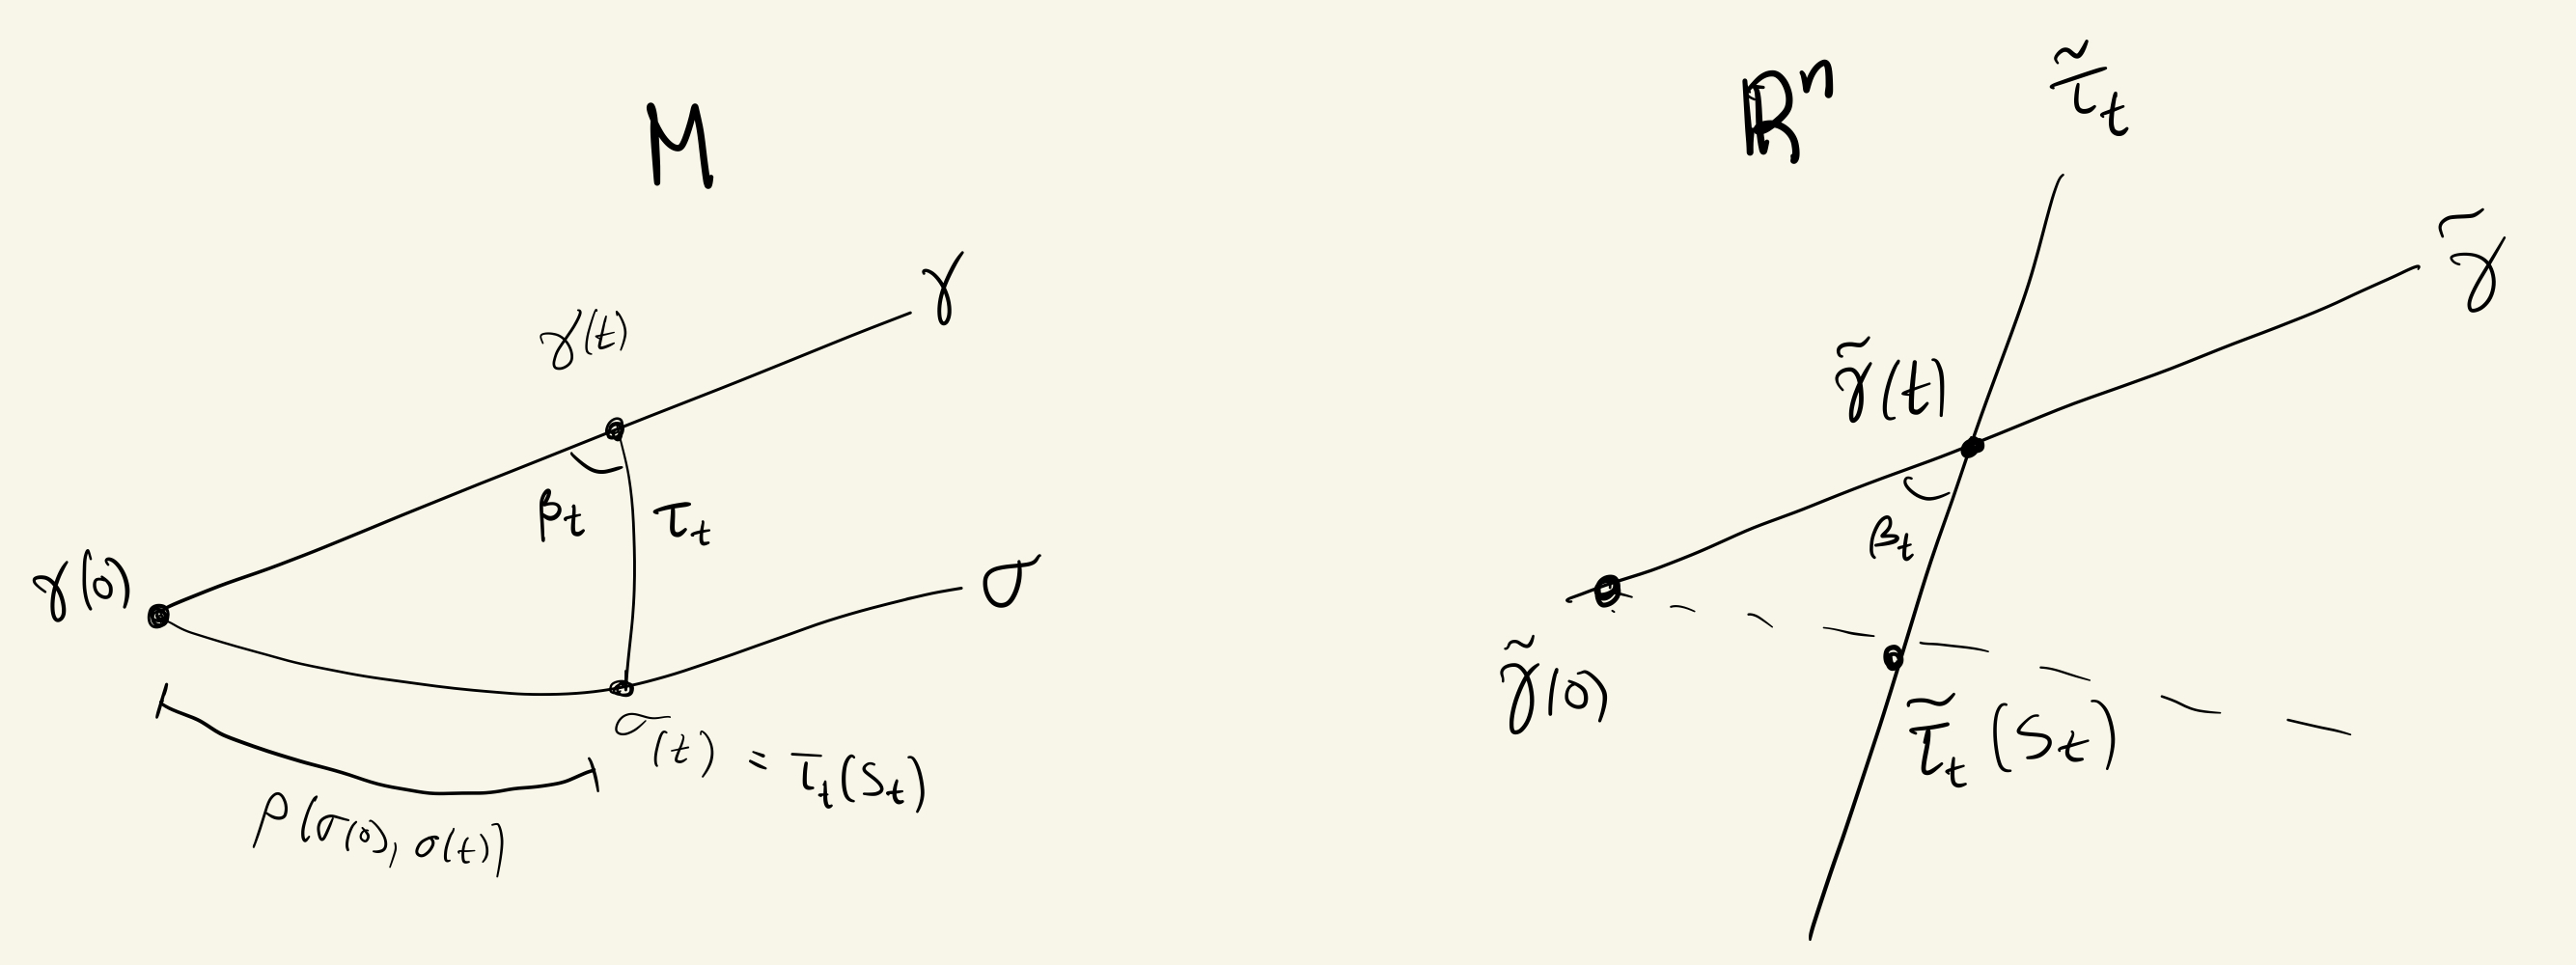
\includegraphics[width=1\textwidth]{figures/toponogov-exercise}
\end{figure}


Como $\tilde{\sigma}$ é uma geodésica no $\mathbb{R}^n$, a distância
 $\rho_{\mathbb{R}^n}(\tilde{\sigma}(0),\tilde{\sigma}(t))$ diverge conforme
 $t\to \infty$, e obtemos o resultado.
\end{proof}



\clearpage
\bibliography{my}
\bibliographystyle{amsalpha}

\end{document}

